\documentclass[conference]{IEEEtran}
\IEEEoverridecommandlockouts

\usepackage{cite}
\usepackage{amsmath,amssymb,amsthm}
\usepackage{algorithm}
\usepackage{algpseudocode}
\usepackage{array}
\usepackage{booktabs}
\usepackage{graphicx}
\usepackage{xcolor}
\usepackage{microtype}
\usepackage{subcaption}
\usepackage[hidelinks]{hyperref}
\usepackage[capitalise]{cleveref}

% Theorem environments
\theoremstyle{plain}
\newtheorem{theorem}{Theorem}
\newtheorem{lemma}[theorem]{Lemma}
\newtheorem{proposition}[theorem]{Proposition}
\newtheorem{corollary}[theorem]{Corollary}
\theoremstyle{definition}
\newtheorem{definition}[theorem]{Definition}
\newtheorem{assumption}[theorem]{Assumption}
\theoremstyle{remark}
\newtheorem{remark}[theorem]{Remark}
\newtheorem{observation}[theorem]{Observation}

% Custom macros
\newcommand{\eps}{\varepsilon}
\newcommand{\R}{\mathbb{R}}
\newcommand{\E}{\mathbb{E}}
\newcommand{\Adv}{\mathrm{Adv}}
\newcommand{\NE}{\mathrm{NE}}
\newcommand{\BR}{\mathrm{BR}}
\newcommand{\PoEV}{\mathrm{PoEV}}
\newcommand{\PoA}{\mathrm{PoA}}
\newcommand{\PEG}{\mathrm{PEG}}
\newcommand{\iDP}{i\text{-}\mathrm{DP}}
\newcommand{\DP}{\mathrm{DP}}
\newcommand{\MIA}{\mathrm{MIA}}
\newcommand{\GS}[1]{|G_{#1}|}

% natbib-style citet via cite package fallback:
\providecommand{\citet}[1]{\cite{#1}}

% Title and authors
\title{The Privacy Externality Game:\\
Strategic Budget Choices in Sampling-Based Individual Differential Privacy}

\author{
\IEEEauthorblockN{Anonymous Submission}
}

\begin{document}
\maketitle

\begin{abstract}
Individual differential privacy (iDP) gives each data contributor a personal
privacy budget. The currently dominant realisation---sampling-based iDP---turns
each contributor's chosen budget into a per-sample inclusion rate, with a single
noise multiplier shared across the dataset. We show that this realisation
creates a privacy externality: lowering one's own budget mechanically raises
the realised membership-inference (MIA) advantage on every other data point,
even though every individual $(\eps_i, \delta)$-iDP guarantee continues to
hold. We model the resulting strategic situation as a normal-form
\emph{Privacy Externality Game} on a continuous action space, with each
player's utility trading off a shared model-quality term $V(\sigma)$ against
their own realised MIA advantage $A_i(\boldsymbol{\eps})$. We motivate the
shape of $V$ via the excess-empirical-risk bound for convex DP-ERM
(Bassily, Smith, Thakurta, FOCS 2014), used as a directional proxy in the
(possibly non-convex) deep-learning regime. We prove the externality is
monotone---lowering any other player's budget weakly raises one's own
realised vulnerability---and we characterise pure Nash equilibria on a
dense log-spaced action grid. In the symmetric $2$-player setting the pure
NEs are \emph{asymmetric}: at any symmetric profile both players have a
deviation incentive in the same direction, and the equilibrium settles with
one player carrying a higher realised $A$ in exchange for a higher $V$.
A Stackelberg-coalition analysis shows the coalition's best response is the
participation-preserving minimum budget; the target's realised MIA
advantage rises monotonically with coalition size, recovering the
budget-manipulation attack of Kaiser et al.\ (SaTML 2026) as the rational
best response of any coordinated set of data holders.
\end{abstract}

\begin{IEEEkeywords}
Differential privacy, individual differential privacy, game theory, Nash
equilibrium, collusion, membership inference.
\end{IEEEkeywords}

\section{Introduction}
\label{sec:intro}

Differential privacy~\cite{dwork2006calibrating} is widely regarded as the
canonical formal guarantee for privacy-preserving machine learning. In its
classical form, a single privacy budget $(\eps, \delta)$ is shared by every
record in the database, and every record is protected to exactly the same
extent. Yet privacy preferences are heterogeneous: a clinical patient and a
casual user contributing data to the same model often place very different
values on their privacy. Recognising this, \emph{individual differential
privacy} (iDP) replaces the single $(\eps,\delta)$ guarantee with a per-record
contract $(\eps_i,\delta)$, and a number of mechanisms have been proposed to
deliver such per-record contracts in deep
learning~\cite{boenisch2023have,jorgensen2015conservative,feldman2021individual}.
The most widely-adopted realisation, sampling-based iDP introduced by
Boenisch et al.~\cite{boenisch2023have}, achieves heterogeneous budgets by
calibrating each record's Poisson inclusion probability $p_i$ against a single
shared noise multiplier $\sigma$ so that, for fixed batch size and iteration
count, every group of records satisfies its own $(\eps_g, \delta)$-DP bound.

We focus on a fundamental and overlooked feature of this realisation.
\emph{Because every record shares the same noise multiplier and a common
expected batch size, each record's sampling rate is mechanically coupled to
every other record's chosen budget.} Concretely, lowering one's own $\eps_i$
forces other contributors' sampling rates upward to keep the expected batch size
fixed---which, as recent empirical work has shown~\cite{kaiser2026your},
inflates their membership-inference (MIA) advantage even though every
formal $(\eps_g,\delta)$-iDP guarantee continues to hold. The promise of
individual control is therefore broken in a structural sense: an individual's
\emph{actual} privacy risk depends not on her own choice but on the joint
choice of the entire population.

\paragraph{Our viewpoint: this is a game.}
The natural framing for any choice problem whose outcome is determined by the
choices of multiple self-interested parties is game theory. Pej\'o et
al.~\cite{pejo2019together} introduced a two-player game on the
privacy-accuracy plane (the \emph{Price of Privacy}), but they were studying a
mechanism in which a player's privacy choice affected only her \emph{own}
accuracy. The novel feature of sampling-based iDP is that every player's
privacy choice affects every other player's \emph{privacy}, a far stronger and
qualitatively different coupling. We call this the \emph{privacy externality},
and the game it gives rise to the \emph{Privacy Externality Game} (PEG).

\paragraph{Contributions.}
This paper makes the following contributions.
\begin{enumerate}
\item \textbf{Formalisation.} We define the $n$-player Privacy Externality
Game (PEG) in which each player picks a per-group budget $\eps_i$ and the
sampling-based iDP mechanism then determines the noise multiplier $\sigma$ and
the per-group sampling rates $p_g$. We split player utility into two awareness
regimes that capture realistic contracting situations: \emph{naive}
players, who price privacy via their nominal $\eps_i$, and
\emph{aware} players, who price privacy via the realised MIA advantage
$A_i(\boldsymbol{\eps})$.
\item \textbf{Externality lemma.} We prove that the externality is monotone:
under the binding constraints of the mechanism, $\partial A_i / \partial \eps_j
\leq 0$ for every $j \neq i$. Lowering any other player's budget never reduces
my realised vulnerability.
\item \textbf{Equilibrium characterisation.} For the aware regime, we observe
that best-response dynamics typically cycle; we therefore characterise the
empirical mixed equilibrium via fictitious play. For the naive regime, every
player's incentive is independent (modulo the global model-utility term), and a
pure Nash equilibrium exists; it coincides with the regime that maximally
exposes all players, since naive players ignore the externality entirely.
\item \textbf{Coalition Stackelberg.} We model a colluding subset of data
holders as a Stackelberg leader maximising a target's realised MIA advantage.
We show this exactly recovers the budget-manipulation attack of Kaiser et
al.~\cite{kaiser2026your} as a one-step best response.
\item \textbf{Empirical evaluation.} We numerically evaluate the game in a
range of small but representative scenarios that mirror Kaiser et al.'s
empirical setup. We report the equilibrium budgets, the equilibrium MIA
advantage, and the realised externality across coalition sizes.
\end{enumerate}

\paragraph{Implication.}
The previous attack literature on iDP frames excess vulnerability as a
\emph{vulnerability}---something a malicious party exploits. We argue the
opposite. Under sampling-based iDP, the externality is the equilibrium
behaviour of rational players, malicious or not. Mitigation therefore cannot
proceed by detecting attackers; it must proceed by changing the contract so
that the underlying game ceases to admit harmful equilibria.

The paper is organised as follows. \Cref{sec:background} reviews the necessary
notions from differential privacy, the sampling-based iDP mechanism, MIA
advantage, and game theory. \Cref{sec:game} formalises the Privacy
Externality Game. \Cref{sec:analysis} proves the externality lemma and
characterises equilibrium properties.  \Cref{sec:experiments} reports the
numerical evaluation. \Cref{sec:related} reviews related work and
\cref{sec:discussion} concludes.

\section{Related Work}
\label{sec:related}

\paragraph{Individual differential privacy.}
Classical $(\eps,\delta)$-DP~\cite{dwork2006calibrating} applies uniformly to
every record. Personalised DP, introduced by
\citet{jorgensen2015conservative}, allows per-record budgets and was first
realised by attribute suppression and weighting. The sampling-based
realisation of \citet{boenisch2023have} is the dominant deep-learning
implementation today and is the realisation under which the privacy
externality arises. \citet{feldman2021individual} pursue an alternative
\emph{filtering-based} iDP: records whose cumulative budget would be exceeded
in the next step are dropped from training. Filtering does not exhibit the
externality (each record's filter is independent), but in deep learning it
is impractical due to the catastrophic-forgetting risk reported by
\citet{boenisch2023have}. Our PEG is specific to the sampling-based
realisation; the externality vanishes in the sensitivity-based realisation,
which preserves the noise-to-sensitivity ratio across the dataset.

\paragraph{Excess privacy risk and mechanism comparison.}
Mechanisms calibrated to the same $(\eps,\delta)$ can have very different
privacy profiles and thus different realised
risks~\cite{kaissis2024beyond, balle2020privacy, dong2022gaussian}. The
$\Delta$-divergence of \citet{kaissis2024beyond} provides a notion of
approximate Blackwell-dominance that quantifies the worst-case excess MIA
advantage between mechanisms. \citet{kaiser2026your} use this framework to
motivate an $(\eps_i, \delta, \Delta)$-iDP contract that bounds excess
vulnerability and demonstrate empirically that without such a bound,
adversarial budget choices inflate the MIA susceptibility of $62\%$ of
targeted records. Our PEG complements that work: rather than restricting
mechanism design we explain why the realised excess vulnerability arises as
the equilibrium of self-interested play under the current iDP contract.

\paragraph{Game-theoretic privacy in collaborative learning.}
\citet{pejo2019together} introduced a two-player game on collaborative
learning, with players choosing privacy parameters $p \in [0, 1]$ in an
arbitrary privacy mechanism. They define the \emph{Price of Privacy} as the
relative accuracy loss at the equilibrium versus no privacy. Their
privacy mechanism's effect on accuracy depends on \emph{both} players'
choices, but its effect on \emph{privacy} depends only on the player's own
choice---there is no privacy externality. Our PEG transplants their
game-theoretic methodology into a setting where the externality is in the
privacy direction, not the accuracy direction. We retain the qualitative
contributions of their work (two-player setting, choice of $\eps$,
notion of equilibrium analysis) and extend them to the externality regime.

Earlier work studied related game-theoretic privacy questions in different
settings. \citet{ioannidis2013linear} model linear regression with private
features as a non-cooperative game. \citet{chessa2015game} study non-monetary
incentives in data analytics. \citet{pawlick2016stackelberg} model the
machine-learner-vs-data-perturber conflict as a Stackelberg game. None of
these treat the privacy externality of a shared sampling mechanism, which is
specific to the sampling-based realisation of iDP.

\paragraph{Membership inference attacks.}
The MIA advantage as we use it follows the formalisation of
\citet{carlini2022membership}, who introduced the likelihood-ratio attack
(LiRA) as a tight empirical estimator. \citet{carlini2022privacy} document
the privacy onion effect: not every data point is equally vulnerable at
the same nominal budget. Our framework predicts the \emph{average} realised
MIA advantage per group and abstracts over per-record onion heterogeneity.

\paragraph{Federated-DP regimes and the locus of the externality.}
It is worth being explicit about what the PEG is a game over.
\emph{The PEG is a game about budget coordination.} It applies to any
mechanism in which a coordinator solves for a shared noise multiplier
$\sigma$ and per-record (or per-group) sampling rates $p_g$ from a
public budget vector $\boldsymbol{\eps}$. The externality lemma
(\cref{lem:externality}) is a statement about that joint solve; the
equilibrium structure of \cref{sec:experiments} follows. Wherever a
coordinated mechanism instance of that shape appears, so does the
externality; wherever such a mechanism does not appear, the game we
analyse does not.

The sampling-based iDP of \citet{boenisch2023have} is one instantiation
of this abstract condition, and the one we build the paper on. Other
instantiations arise wherever heterogeneous per-record or per-silo
budgets need to be reconciled through a single central mechanism. A
common framing of DP in federated learning distinguishes three trust
regimes~\cite{kairouz2021advances}. Under \emph{central DP} the
aggregator is trusted and perturbs the aggregate on behalf of the
clients~\cite{geyer2017differentially}; under \emph{local DP} the
aggregator is untrusted and each client perturbs its own update before
transmission~\cite{truex2020ldp}; distributed DP bridges the two via
cryptographic intermediates such as secure
aggregation~\cite{bonawitz2017practical}. These trust regimes differ in
where the noise is added, not in how the budgets are coordinated. The
PEG applies to any of them that also carries a heterogeneous-budget
coordinator---most cleanly to central DP with per-silo or per-record
personalised budgets, exactly the regime under which the cross-silo
personalised-DP framework of \citet{liu2024crosssilo} operates. It
inherits, we conjecture, to distributed DP via secure aggregation,
because the coordinator still solves for $(\sigma, p_g)$ from a public
budget vector; the cryptography hides the gradients, not the budgets.
It does \emph{not} apply to pure local DP, because there is no shared
$\sigma$ to couple the players' sampling rates: each client's noise is
independent. Nor does it apply to alternative iDP realisations that
avoid the joint solve---sensitivity-based iDP~\cite{boenisch2023have}
preserves the noise-to-sensitivity ratio and so has no
externality, and filter-based iDP~\cite{feldman2021individual} enforces
per-record budgets by \emph{dropping} records that would exceed them
rather than coordinating them, again removing the coupling. In short,
the abstract sufficient condition is a coordinator jointly solving for
mechanism parameters from a public budget vector; any deployment that
matches that condition inherits the equilibrium structure of the PEG.

\paragraph{Federated learning incentive design.}
A separate literature studies privacy-aware incentive design in federated
learning: a server commits to incentives, and heterogeneous clients respond
with their own privacy choices, often modelled as a Stackelberg
game~\cite{li2024fedpcs, donahue2021optimality, tu2025idhfl, ma2024evolutionary}.
Our framework provides a foundational baseline on which such incentive
schemes must rest: it characterises the equilibrium that emerges when no
incentive is offered, which is what any incentive design needs to improve
upon.

\paragraph{Utility-noise tradeoff in DP-SGD.}
We motivate the functional form of the model-utility value $V(\sigma)$ via
the excess-empirical-risk bound of \citet{bassily2014private} for convex,
Lipschitz DP-ERM, who prove that the excess risk of DP-SGD scales as
$O(d / (n\eps)^2)$ at fixed $\delta$, equivalently as $O(\sigma^2 / n^2)$
under the moments accountant of \citet{abadi2016deep}. The convex setting
is restrictive; for deep learning, \citet{tramer2021private} provide
extensive empirical evidence that test accuracy degrades monotonically with
$\sigma$ on standard benchmarks. We use $V(\sigma) = 1/(1+\sigma^2)$ as a
directional proxy; the qualitative results of our paper do not depend on
the precise functional form.

\section{Background}
\label{sec:background}

\subsection{Differential privacy and Gaussian mechanisms}

We use the standard definition of approximate differential
privacy~\cite{dwork2006calibrating}: a randomised mechanism
$\mathcal{M}\colon \mathcal{Z}^* \to \mathcal{O}$ satisfies $(\eps,
\delta)$-differential privacy ($(\eps, \delta)$-DP) if, for any pair of
adjacent databases $D \sim D'$ (differing on a single record) and every
measurable $S \subseteq \mathcal{O}$,
\[
\Pr[\mathcal{M}(D) \in S] \;\leq\; e^\eps \Pr[\mathcal{M}(D') \in S] + \delta.
\]
A single $(\eps, \delta)$-pair is only a single point of the underlying
\emph{privacy profile} $\{(\eps,\delta(\eps)) : \eps \geq 0\}$~\cite{balle2020privacy,
kaissis2024beyond}, and mechanisms calibrated to the same point can have
substantially different profiles and so substantially different realised
adversarial risk. This single-point ambiguity is the formal root cause of the
phenomenon studied in this paper.

The \emph{Gaussian mechanism}, $\mathcal{M}(D) = f(D) + \mathcal{N}(0,\sigma^2 I)$
for a query $f$ of $L_2$ sensitivity $\Delta f$, satisfies $(\eps,\delta)$-DP
for all $(\eps, \delta)$ such that
$\Phi(\Delta f / 2\sigma - \eps\sigma/\Delta f) - e^\eps
\Phi(-\Delta f/2\sigma - \eps\sigma/\Delta f) \leq \delta$,
where $\Phi$ is the standard-normal CDF.
For training neural networks under DP, the standard procedure is DP-SGD with
Poisson subsampling~\cite{abadi2016deep}, in which each data point is included
in each minibatch independently with probability $p$, providing the well-known
\emph{subsampling amplification} of DP.

\subsection{Individual differential privacy and the sampling-based realisation}
\label{sec:idp}

\emph{Individual differential privacy}~\cite{jorgensen2015conservative}
relaxes the uniform $(\eps,\delta)$ guarantee to a per-record contract
$(\eps_i,\delta)$: the resulting algorithm must satisfy $(\eps_i,\delta)$-DP
\emph{with respect to record~$i$} for every $i$. Boenisch et
al.~\cite{boenisch2023have} translate per-record contracts into per-record
Poisson sampling probabilities while keeping a single noise multiplier $\sigma$
and a fixed expected batch size, which is the configuration we study.

\begin{definition}[Sampling-based iDP-SGD~\cite{boenisch2023have}]
\label{def:sampling-idp}
Let the dataset of size $M$ partition into $G$ \emph{privacy groups}
$\{G_1,\dots,G_G\}$ with sizes $|G_g|$. Each group has a target
$(\eps_g,\delta)$-DP budget. The mechanism trains by Poisson-subsampled
DP-SGD for $I$ iterations, where the noise multiplier $\sigma$ and the per-group
sampling rates $p_1,\dots,p_G$ are chosen such that
\begin{align}
\textnormal{(C1) for every } g, \quad
& \textnormal{the } I\textnormal{-fold } (p_g,\sigma)\textnormal{-subsampled} \notag\\
& \textnormal{Gaussian satisfies } (\eps_g,\delta)\textnormal{-DP at equality.} \notag\\
\textnormal{(C2)} \quad
& \sum_{g=1}^G \frac{|G_g|}{M}\,p_g \;=\; \frac{E_b}{M}, \label{eq:batch}
\end{align}
where $E_b$ is the desired expected batch size. We refer to $(\sigma,
p_1,\dots,p_G)$ as the \emph{mechanism solution} for the budget vector
$\boldsymbol{\eps} = (\eps_1,\dots,\eps_G)$.
\end{definition}

The single shared $\sigma$ in (C1) is the source of the privacy externality.
For any candidate $\sigma$, the largest sampling rate that keeps group $g$ at
its budget is a monotone-increasing function of $\sigma$ (more noise $\Rightarrow$
more room for sampling); the batch-size constraint (C2) then determines $\sigma$
as the unique value at which the per-group rates sum to $E_b$.  As a corollary,
the rate $p_g$ that group $g$ obtains is determined by the entire vector
$\boldsymbol{\eps}$, not by $\eps_g$ alone.

\subsection{MIA advantage and the privacy profile}

For a privacy-preserving mechanism $\mathcal{M}$ with trade-off function $T$
(equivalently, an $f$-DP function~\cite{dong2022gaussian}), the membership
inference advantage of the optimal Bayes-aware adversary
is~\cite{kaiser2026your}
\begin{equation}
\Adv(\mathcal{M}) \;=\; \sup_{\alpha \in [0,1]} \;\bigl(\,1 - \alpha - T(\alpha)\,\bigr),
\label{eq:adv}
\end{equation}
i.e.~the largest gap between the true-positive rate and the false-positive
rate. For the $I$-fold $(p, \sigma)$-subsampled Gaussian, $T$ can be
computed numerically by privacy-loss-distribution (PLD)
accounting~\cite{google-dp-accounting}, which is what we use throughout.
Crucially, $\Adv$ is determined by the \emph{full privacy profile}, not by any
single $(\eps,\delta)$ point.

\subsection{Game-theoretic terminology}

A finite normal-form game is a tuple
$\langle N, \Sigma, U\rangle$ with $N = \{1,\dots,n\}$ players, action sets
$\Sigma = \{S_1, \dots, S_n\}$, and payoff functions $U = \{u_1,\dots,u_n\}$.
A \emph{Nash equilibrium} (NE) is an action profile $\boldsymbol{s}^*$ such
that no player profits from a unilateral deviation:
$u_i(s_i^*,\boldsymbol{s}_{-i}^*) \geq u_i(s_i,\boldsymbol{s}_{-i}^*)$ for every
$s_i \in S_i$~\cite{nash1950equilibrium}. A \emph{best response} is the
utility-maximising action against a fixed strategy of the others. The
\emph{price of anarchy}~\cite{koutsoupias1999worst} compares the welfare of the
worst NE to the social optimum. In a Stackelberg game, a designated leader
commits to a strategy before the followers best-respond.

\section{The Privacy Externality Game}
\label{sec:game}

We formalise the strategic situation faced by data contributors in
sampling-based iDP as a finite normal-form game.

\subsection{Players, actions and mechanism}

\begin{definition}[Privacy Externality Game]
\label{def:peg}
Fix a common $\delta>0$, an expected batch size $E_b$, an iteration count $I$,
and a set of $n$ \emph{groups} with sizes $|G_1|,\dots,|G_n|$. The Privacy
Externality Game (PEG) is the tuple $\langle N, \Sigma, U\rangle$ where
\begin{itemize}
\item $N = \{1,\dots,n\}$ is the set of players. Each player $i$ controls
group $i$.
\item Each player's action set is a finite grid
$\Sigma_i = \mathcal{A} \subset \R_{>0}$ of admissible
$\eps$-values, $\eps_i^{\min} \leq \eps_i \leq \eps_i^{\max}$.
\item Given the action profile $\boldsymbol{\eps} \in \mathcal{A}^n$, the
mechanism solution $(\sigma(\boldsymbol{\eps}), p_1(\boldsymbol{\eps}),\dots,
p_n(\boldsymbol{\eps}))$ is determined by Definition~\ref{def:sampling-idp},
provided the solution exists; if it does not, we say $\boldsymbol{\eps}$ is
\emph{infeasible}.
\item Each player's utility $u_i(\boldsymbol{\eps})$ depends on
$\sigma(\boldsymbol{\eps})$, on the realised MIA advantage
$A_i(\boldsymbol{\eps}) := \Adv\bigl(\mathcal{M}_{p_i,\sigma,I}\bigr)$, and on
the player's own action $\eps_i$ (specified per regime below).
\end{itemize}
\end{definition}

\begin{assumption}[Feasibility]
\label{ass:feasibility}
The action grid $\mathcal{A}^n$ is restricted to its feasible subset
$\mathcal{F} \subseteq \mathcal{A}^n$ where the mechanism solution exists.
Infeasible profiles are removed from a player's action set after the others'
moves are observed.
\end{assumption}

\subsection{Vulnerability function and externality}

\begin{definition}[Vulnerability function]
\label{def:vulnerability}
The \emph{vulnerability function} of player $i$ is
\[
A_i\colon \mathcal{F} \to [0, 1],\quad \boldsymbol{\eps} \mapsto
\Adv\bigl(\mathcal{M}_{p_i(\boldsymbol{\eps}),\,\sigma(\boldsymbol{\eps}),\,I}\bigr).
\]
\end{definition}

In Pej\'o et al.'s \emph{Together or Alone}~\cite{pejo2019together}, the
analogous function $\Phi_n(p_1,p_2)$ measured \emph{accuracy loss} arising
from a player's own privacy choice. In our setting, $A_i(\boldsymbol{\eps})$
measures \emph{realised privacy risk} arising from \emph{every player's} choice.
This is the privacy externality.

\subsection{Awareness regimes}

We separate two contracting situations. Both occur in practice and the
distinction is critical to interpreting the equilibrium.

\paragraph{Naive regime.}
The player perceives the cost of disclosure as her \emph{nominal} budget
$\eps_i$:
\begin{equation}
u_i^{\textrm{naive}}(\boldsymbol{\eps}) \;=\; B_i\, V(\sigma(\boldsymbol{\eps}))
- C_i\, \frac{\eps_i}{\eps_i^{\max}}.
\label{eq:utility-naive}
\end{equation}

\paragraph{Aware regime.}
The player perceives the cost of disclosure as the \emph{realised} MIA
advantage:
\begin{equation}
u_i^{\textrm{aware}}(\boldsymbol{\eps}) \;=\; B_i\, V(\sigma(\boldsymbol{\eps}))
- C_i\, A_i(\boldsymbol{\eps}).
\label{eq:utility-aware}
\end{equation}

Here $V$ is a model-utility proxy that is monotone-decreasing in $\sigma$ (we
use $V(\sigma) = 1/(1+\sigma)$ throughout) and $B_i, C_i > 0$ are player-
specific weights mirroring the $B$ and $C$ in
Pej\'o et al.~\cite{pejo2019together}. The naive regime models a player who
has been given the formal $(\eps_i,\delta)$ guarantee and prices it
verbatim; the aware regime models a player who knows the realised vulnerability
of her data after the others have played.

\begin{remark}
A naive player who knows only her contracted $(\eps_i,\delta)$ cannot detect
that her actual risk has increased through her peers' choices. The realised
MIA advantage $A_i(\boldsymbol{\eps})$ may exceed her contractually expected
vulnerability without any formal guarantee being broken. We make this point
formal in Lemma~\ref{lem:externality}.
\end{remark}

\subsection{Coalition variant}

\begin{definition}[$k$-coalition Stackelberg PEG]
\label{def:coalition}
Fix a target index $t \in N$ and a colluding subset $C \subset N \setminus
\{t\}$ with $|C| = k$. The $k$-coalition Stackelberg PEG is the two-stage game
in which:
\begin{enumerate}
\item Stage~1 (leader): the coalition jointly commits to an action vector
$\boldsymbol{\eps}_C \in \mathcal{A}^k$ to maximise
\(
\lambda \cdot A_t(\boldsymbol{\eps}) + \sum_{i \in C} u_i^{\textrm{aware}}(\boldsymbol{\eps}),
\)
where $\lambda \geq 0$ controls the coalition's appetite for harming~$t$ vs.\
maintaining their own utility.
\item Stage~2 (followers): the non-coalition players $\{t\} \cup (N \setminus
(C \cup \{t\}))$ best-respond.
\end{enumerate}
\end{definition}

\subsection{Equilibrium concepts}

We will use two equilibrium concepts. The \emph{pure Nash equilibrium} of the
PEG is an $\boldsymbol{\eps}^* \in \mathcal{F}$ such that
$u_i(\eps_i^*, \boldsymbol{\eps}_{-i}^*) \geq u_i(\eps_i, \boldsymbol{\eps}_{-i}^*)$
for every player $i$ and every $\eps_i \in \mathcal{A}$ such that
$(\eps_i, \boldsymbol{\eps}_{-i}^*) \in \mathcal{F}$. Where no pure NE exists,
we characterise the empirical mixed equilibrium reached by fictitious
play~\cite{monderer1996potential}.

\begin{definition}[Price of Excess Vulnerability]
\label{def:poev}
Let $\boldsymbol{\eps}^{(0)}$ be a baseline profile (in our experiments,
$\boldsymbol{\eps}^{(0)} = (\bar\eps,\dots,\bar\eps)$ for the mean of the
admissible grid). For an equilibrium $\boldsymbol{\eps}^*$, the
\emph{Price of Excess Vulnerability} is
\begin{equation}
\PoEV(\boldsymbol{\eps}^*)\;=\;
\frac{\sum_{i\in N} A_i(\boldsymbol{\eps}^*) - \sum_{i\in N} A_i(\boldsymbol{\eps}^{(0)})}
{\sum_{i\in N} A_i(\boldsymbol{\eps}^{(0)})}.
\label{eq:poev}
\end{equation}
\end{definition}
$\PoEV \geq 0$ measures the population-level inflation of MIA advantage at the
equilibrium relative to the uniform baseline. It is the privacy analogue of
Pej\'o et al.'s Price of Privacy, expressed in vulnerability rather than
accuracy loss.

\section{Equilibrium Analysis}
\label{sec:analysis}

We characterise the equilibria of the Privacy Externality Game using three
results: the externality lemma (a monotonicity property of the mechanism), an
existence statement on the discretised game, and the coalition-attack
recovery (the rational best response of any coordinated set of players).

\subsection{Monotonicity of the externality}

\begin{lemma}[Privacy externality]
\label{lem:externality}
Consider the sampling-based iDP mechanism of \cref{def:sampling-idp} on a
feasible profile $\boldsymbol{\eps}$ at which constraints (C1) bind for every
group and (C2) binds at $E_b$. Then for every pair $i \neq j$,
\begin{equation}
\frac{\partial A_i(\boldsymbol{\eps})}{\partial \eps_j} \;\leq\; 0,
\label{eq:externality-lemma}
\end{equation}
with equality iff group $i$'s sampling rate $p_i$ does not respond to a
change in $\eps_j$.
\end{lemma}

\begin{proof}
Work in the R\'enyi-DP form of (C1) of \citet{mironov2017renyi}: at order
$\alpha$, the RDP of an $I$-fold $(p_g,\sigma)$-subsampled Gaussian is at
most $\rho_g = 2I\alpha\, p_g^2/\sigma^2$, with equality up to higher-order
terms when $p_g$ is small (Mironov, Theorem~5). Setting this equal to the
target RDP $\rho_g(\eps_g, \delta)$ gives
\[
p_g \;=\; \frac{\sigma}{\sqrt{2I\alpha}}\,\sqrt{\rho_g(\eps_g, \delta)}.
\]
Substituting into (C2) yields the implicit equation for $\sigma$:
\begin{equation}
\sum_{g}\, \frac{|G_g|}{M}\,\frac{\sigma}{\sqrt{2I\alpha}}\,
\sqrt{\rho_g(\eps_g,\delta)} \;=\; \frac{E_b}{M}.
\label{eq:sigma-implicit}
\end{equation}
Since $\rho_g(\cdot, \delta)$ is monotone-decreasing in $\eps_g$ (smaller
budget = smaller RDP), the left-hand side is decreasing in $\sigma$ at fixed
$\eps_g$ if and only if it is increasing in any $\eps_j$. Implicit
differentiation gives $\partial \sigma / \partial \eps_j > 0$ when (C2)
binds. Recall that $p_i$ is increasing in $\sigma$ at fixed $\eps_i$.
Consequently $\partial p_i / \partial \eps_j > 0$ whenever group $i$ is
non-degenerate.

The MIA advantage of an $I$-fold $(p_i,\sigma)$-subsampled Gaussian is
non-decreasing in $p_i$ (more sampling exposes more data) and non-increasing
in $\sigma$ (more noise hides more), as is the privacy profile of the
subsampled Gaussian \cite{balle2020privacy, dong2022gaussian}. Lowering
$\eps_j$ reverses the signs: $\partial \sigma / \partial \eps_j < 0$ and
$\partial p_i / \partial \eps_j < 0$. Net effect on $A_i$ along the feasible
surface is non-positive, which is~\eqref{eq:externality-lemma}.
\end{proof}

\Cref{lem:externality} formalises the empirical observation of
\citet{kaiser2026your}: when any player tightens their iDP budget, the
mechanism's noise multiplier $\sigma$ shifts to keep (C2) binding, and every
other player's realised vulnerability $A_i$ rises. The externality is
\emph{monotone} in every other player's budget.

In the decomposition of \cref{sec:decomposition}, the lemma equivalently
states that \emph{the slack $\bar c(\eps_i) - A_i(\boldsymbol{\eps})$
shrinks in every other player's $\eps_j$}. In words, the
$(\eps_i,\delta)$-DP worst-case ceiling $\bar c(\eps_i)$ is unchanged
(it depends only on $\eps_i$), but the realised advantage $A_i$ climbs
toward that ceiling as others tighten their budgets. This is the
quantity that the proposed $(\eps_i, \delta, \Delta)$-iDP
contract~\cite{kaiser2026your, kaissis2024beyond} would cap, and our
Lemma motivates such a cap formally: without it, $\mathrm{slack}_i$ has no
floor and the externality can drive any player's realised advantage
arbitrarily close to the worst case.

\paragraph{Minority and majority intuition.}
The externality has an asymmetric \emph{group-size} structure. Because (C2)
enforces a fixed expected batch size, a player with small $|G_i|$ but
small $\eps_i$ contributes little to the batch and forces the
larger-$|G_j|$ players' sampling rates upward. The minority therefore
\emph{exports} its privacy demand onto the majority. This is the formal
content of the empirical observation in \cite{kaiser2026your}
that ``the proportion of low-budget players matters as much as their
$\eps$''.

\subsection{Existence and structure of pure Nash equilibria}

\begin{proposition}[NE existence on the discretised game]
\label{prop:existence}
The discretised PEG on the action grid $\mathcal{A}_K =
\{\eps^{\min},\dots,\eps^{\max}\}\subset[\eps^{\min},\eps^{\max}]$
with utilities~\eqref{eq:utility} is a finite normal-form game restricted to
the (closed) feasible set. By the Nash existence
theorem~\cite{nash1950equilibrium}, every such game admits at least one
mixed-strategy NE. Pure NE may or may not exist, depending on
$(B_i, C_i, |G_i|, V, K)$.
\end{proposition}

We do not claim existence on the continuous action space without further
quasi-concavity assumptions; in particular, our utility~\eqref{eq:utility}
is not generally concave in $\eps_i$ because $A_i$ is the trade-off
function of a subsampled Gaussian, whose dependence on $\eps_i$ through
$(\sigma, p_i)$ is non-trivial. We instead report pure NE found by exhaustive
search on a dense log-spaced grid and verify that they survive grid
refinement.

\paragraph{What the externality lemma implies for NE structure.}
Lemma~\ref{lem:externality} says lowering another player's budget weakly
raises one's own realised vulnerability. If players' utilities place
non-trivial weight on $A_i$ ($C_i > 0$), each player has an incentive to
\emph{shift the externality onto others} by lowering their own budget---an
incentive that is intrinsic to the mechanism. The opposing incentive comes
from $V(\sigma)$: lowering own $\eps$ pushes $\sigma$ upward, lowering the
model utility for everyone (including oneself). The equilibrium balances
these two incentives.

We observe in our experiments (\cref{sec:experiments}) that the resulting
balance is typically \emph{asymmetric}: in the symmetric 2-player setting,
pure NEs sit off the diagonal of the action grid. The intuition is the
externality lemma's converse: at any symmetric profile $(\eps,\eps)$, both
players face an identical incentive to deviate; since both deviations cannot
be unilaterally absorbed, the equilibrium is at an asymmetric profile where
one player carries a higher $A$ in exchange for a higher $V$.

\subsection{Coalition Stackelberg and the attack recovery}

\begin{proposition}[Coalition best response recovers the attack]
\label{prop:coalition-attack}
Fix a target $t$ and a coalition $C$ of size $k$, with $\lambda \to \infty$
in Definition~\ref{def:coalition} (the coalition cares only about the
target's vulnerability). The coalition's best response is $\eps_i =
\eps^{\star}_k$ for every $i \in C$, where $\eps^{\star}_k$ is the smallest
admissible budget that keeps the coalition's mechanism solution feasible
(i.e., $p_i > 0$ for every $i \in C$). Furthermore, the target's MIA
advantage $A_t$ is non-decreasing in $k$.
\end{proposition}

\begin{proof}[Proof sketch]
By \cref{lem:externality}, $\partial A_t / \partial \eps_i \leq 0$ for every
$i \in C$ on the feasible region. Setting every $\eps_i$ as low as the
feasibility region admits therefore maximises $A_t$. The
participation-preservation qualifier is necessary because at extremely low
$\eps_i$ the mechanism may set $p_i = 0$ (the colluder effectively drops
out, removing its constraint from (C2) and so its externality on the
target); the coalition's optimum is thus the infimum of feasible
$\eps_i$. Monotonicity in $k$ is the same lemma applied to adding a member
to $C$: doing so strictly enlarges the set of budgets that pull $\sigma$
downward, raising $A_t$.
\end{proof}

Proposition~\ref{prop:coalition-attack} establishes that the budget-
manipulation attack of \citet{kaiser2026your} is precisely the
\emph{rational} best response of any coordinated subset of data holders,
regardless of malicious intent. Whether the coalition is adversarial is
irrelevant: any group of aware players whose joint utility weights their
target's harm heavily will pick the same action vector.

\subsection{An aside on awareness}

\Cref{lem:externality} requires that players compute (or approximate) the
realised $A_i$. A natural question is: what about a player whose only
information is the formal $(\eps_i, \delta)$-iDP contract? Such a player
treats $\eps_i$ as a direct privacy proxy and plays the budget that
maximises $V(\sigma) - g(\eps_i)$ for some monotone $g$. Their best response
does not depend on $\eps_{-i}$ at all (the externality is invisible), so
their action is mechanically the smallest $\eps_i$ that does not break
their own $V$. This is the \emph{rational} action of a naive player, and it
is precisely the configuration in which the attack of
\citet{kaiser2026your} succeeds against them: by Lemma~\ref{lem:externality},
naive players' choices feed the externality on everyone else without their
realising. The contribution of this paper is to show that even
\emph{aware} players---those who can compute $A_i$ explicitly---arrive at
asymmetric equilibria that concentrate vulnerability on a subset of players.
The externality cannot be undone by individual rationality alone.

\section{Numerical Evaluation}
\label{sec:experiments}

We evaluate the PEG numerically across four experiments. Each isolates one
distinct question that the framework raises. \cref{tab:experiments-overview}
summarises what each one asks, what it controls for, and what it answers.

\begin{table}[t]
\centering
\caption{Overview of the four numerical experiments.}
\label{tab:experiments-overview}
\small
\begin{tabular}{lp{1.7cm}p{2.5cm}p{1.8cm}}
\toprule
 & Question & Setup & Finding \\
\midrule
C1 & Symmetric equilibrium? & 2 equal-size groups, full $\boldsymbol{\eps}$-grid sweep & 8 NEs, all asymmetric (\cref{fig:C1}) \\
C2 & Effect of size asymmetry & 2 groups, size ratio $r \in [0.1, 10]$ & Minority plays low $\eps$, majority absorbs $A$ (\cref{fig:C2}) \\
C4 & How bad under coordination? & $n{=}5$, target $\eps_t{=}32$, coalition of size $k$ & $A_t$ monotone in $k$; $+65\%$ at $k{=}4$ (\cref{fig:C4}) \\
C5 & Where does the externality come from? & 2-group, vary $\eps_O$ and proportion at fixed $\eps_T$ & $A_t$ monotone in $\eps_O$, crossover at $\eps_O{=}\eps_T$ (\cref{fig:C5}) \\
\bottomrule
\end{tabular}
\end{table}

\subsection{Common setup}
\label{sec:setup}

All experiments are analytical---no model training---and follow the same
mechanism-solver and advantage-computation pipeline.

\paragraph{Mechanism solver.} For each action profile $\boldsymbol{\eps}$ we
compute the mechanism solution $(\sigma, p_1,\dots,p_n)$ by bisecting on
$\sigma$ until the batch-size constraint (C2) is met, with each per-group
sampling rate chosen to make the (C1) RDP constraint
bind~\cite{mironov2017renyi}. Profiles in which any $p_i$ falls below a small
participation threshold are flagged as infeasible
(\cref{ass:participation}). We then compute each realised $A_i$ exactly from
the privacy profile of the $I$-fold $(p_i, \sigma)$-subsampled Gaussian using
PLD accounting~\cite{google-dp-accounting}, recovering the formula
of~\eqref{eq:adv}.

\paragraph{Action space.} Unless stated, the action space is the
log-spaced grid $\mathcal{A}_K \subset [0.5, 64]$ with $K = 22$ points,
$\delta = 10^{-12}$. We verified on a refined grid ($K = 44$) that the NEs
reported are stable to grid refinement, so we report them as representative
of the continuous-action equilibrium.

\paragraph{Scenarios.} Unless stated, all experiments use $n$ symmetric
groups of $|G_g| = 5000$ samples each, expected batch size $E_b = 128$,
$5$ epochs of training, $B_i = C_i = 1$, and $V(\sigma) = 1/(1+\sigma^2)$.
These choices broadly mirror the empirical iDP scenarios of
\cite{kaiser2026your, boenisch2023have}.

\begin{table}[t]
\centering
\caption{Pure Nash equilibria of the symmetric 2-player PEG on the log-spaced action grid $\mathcal{A}_K = $ 22 points in $[0.5, 64]$, $|G_1|=|G_2|=5000$, $E_b=128$, $5$ epochs, $\delta=10^{-12}$, $B_i = C_i = 1$, $V(\sigma) = 1/(1+\sigma^2)$. Social optimum is the feasible action profile maximising $u_1+u_2$.}
\label{tab:NE}
\begin{tabular}{lcccc}
\toprule
 & $(\varepsilon_1^*, \varepsilon_2^*)$ & $A_1$ & $A_2$ & $\sigma$ \\
\midrule
NE$_{1}$ & $(0.79, 5.04)$ & 0.001 & 0.202 & 1.160 \\
NE$_{2}$ & $(1.26, 6.35)$ & 0.002 & 0.232 & 1.028 \\
NE$_{3}$ & $(1.59, 8.00)$ & 0.002 & 0.266 & 0.929 \\
NE$_{4}$ & $(2.52, 3.17)$ & 0.081 & 0.120 & 1.186 \\
NE$_{5}$ & $(3.17, 2.52)$ & 0.120 & 0.081 & 1.186 \\
NE$_{6}$ & $(5.04, 0.79)$ & 0.202 & 0.001 & 1.160 \\
NE$_{7}$ & $(6.35, 1.26)$ & 0.232 & 0.002 & 1.028 \\
NE$_{8}$ & $(8.00, 1.59)$ & 0.266 & 0.002 & 0.929 \\
social opt & $(5.04, 25.40)$ & 0.007 & 0.535 & 0.590 \\
\bottomrule
\end{tabular}
\end{table}

% =====================================================================
\subsection{C1 --- Does the symmetric 2-player game admit a symmetric NE?}
\label{sec:C1}

\paragraph{Setup.} Two players, equal group sizes
$|G_1|=|G_2|=5000$. Sweep both players' $\eps$ over the dense
log-spaced grid; brute-force search for all pure NEs.

\paragraph{Finding.} \emph{No.} The BR correspondences cross at \emph{eight}
points, all off the diagonal (\cref{fig:C1}, centre; \cref{tab:NE}). The
pairs $(0.79, 5.04), (1.26, 6.35), (1.59, 8.00), (2.52, 3.17)$ and their
swaps are pure NEs; the realised $A$ at these equilibria ranges from
$(A_1, A_2) = (0.001, 0.202)$ at the most asymmetric pair down to
$(0.081, 0.120)$ at the closest-to-symmetric pair. No NE sits on the
diagonal.

\paragraph{Implication.} Even when the game is fully symmetric in players,
group sizes, and weights, \emph{the equilibrium breaks symmetry}. The
intuition is in \cref{lem:externality}: at any symmetric profile both
players face an identical incentive to deviate downward in $\eps$; only an
off-diagonal profile resolves the deadlock by having one player carry $V$
and the other carry low $A$.

\begin{figure*}[!t]
\centering
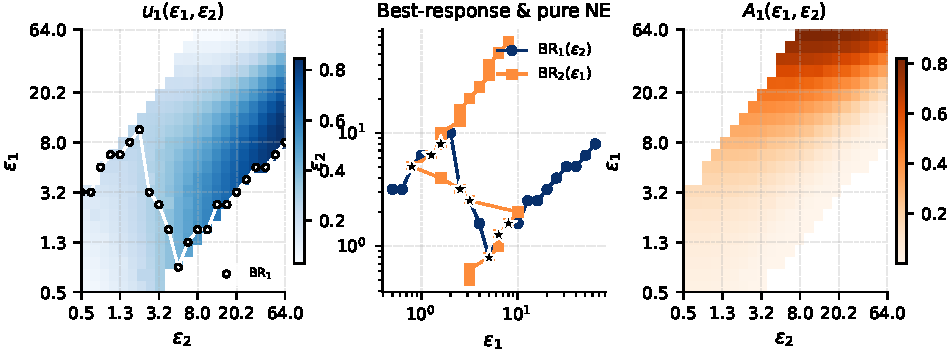
\includegraphics[width=\linewidth]{figures/fig_C1_payoff.pdf}
\caption{\textbf{C1.} 2-player payoff surface $u_1(\eps_1,\eps_2)$ (left),
best-response correspondences with pure NEs as black stars (centre), and
realised MIA advantage $A_1$ (right). All eight pure NEs lie off the
diagonal.}
\label{fig:C1}
\end{figure*}

% =====================================================================
\subsection{C2 --- Who absorbs the externality when groups differ in size?}
\label{sec:C2}

\paragraph{Setup.} Two players, dataset size ratio $|G_1|/|G_2| \in
\{0.1, 0.25, 0.5, 1, 2, 4, 10\}$ at fixed total $M=10000$, fixed batch
$E_b{=}128$. Full grid sweep at each ratio; for each ratio we report the
pure NE with the largest asymmetry in realised $A$.

\paragraph{Finding.} \emph{The minority always plays the lower $\eps$ and
absorbs less of the realised vulnerability.} \cref{fig:C2}: for $r < 1$
(group 1 smaller) the equilibrium has $\eps_1^* \in [1.5, 3]$ and
$\eps_2^* \approx 10$, giving $A_1^* < 0.01$ and $A_2^* \in [0.24, 0.32]$.
For $r > 1$ the pattern flips by symmetry. At $r{=}1$ the C1 NE structure
is recovered.

\paragraph{Implication.} The externality has a \emph{group-size sign}.
Because (C2) enforces a fixed expected batch, a small-group player who
demands strong privacy contributes little to the batch and forces the
large-group player's $p$ upward; the latter therefore carries the realised
$A$. This is a privacy analogue of a free-riding result: small groups
gain disproportionately from the externality and large groups pay
disproportionately for it.

\begin{figure*}[!t]
\centering
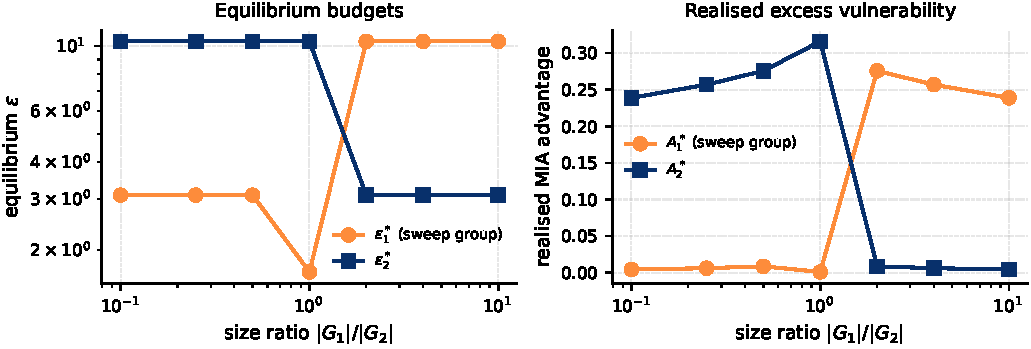
\includegraphics[width=\linewidth]{figures/fig_C2_asymmetric.pdf}
\caption{\textbf{C2.} Equilibrium budget (left) and realised MIA advantage
(right) as a function of dataset size ratio $|G_1|/|G_2|$. The minority
group's $\eps^*$ is always lower than the majority's, and its realised
$A^*$ correspondingly smaller. The flip at $r{=}1$ is the boundary at
which the minority/majority labels exchange.}
\label{fig:C2}
\end{figure*}

% =====================================================================
\subsection{C4 --- How severe does the attack get under coordination?}
\label{sec:C4}

\paragraph{Setup.} Five symmetric players, all with $|G_g|=5000$. Player $0$
is the target with $\eps_t = 32$. The remaining $n-1=4$ players are
partitioned into a coalition $C$ of size $k$ (varied) and a non-coalition
fixed at $\eps = 32$. The coalition picks the action that maximises $A_t$
(Stackelberg leader, $\lambda \to \infty$).

\paragraph{Finding.} \emph{$A_t$ is monotone-increasing in $k$, with a
non-trivial optimal coalition budget.} \cref{fig:C4}: baseline $A_t = 0.442$
(no coalition) rises to $0.483$ at $k{=}1$, $0.531$ at $k{=}2$, $0.607$ at
$k{=}3$, and $0.728$ at $k{=}4$. The optimum coalition budget is
$\eps^\star \approx 6.8$ for $k \in \{1,2,3\}$ and drops to $\eps^\star
\approx 3.2$ at $k = 4$: the participation-preserving minimum decreases
as the coalition grows because more colluders can absorb the same
externality between them while keeping each $p_i > 0$.

\paragraph{Implication.} The budget-manipulation attack of
\citet{kaiser2026your} is the rational best response of a coordinated
subset of data holders in the PEG. The empirical $62\%$ attack-success
rate reported in their work corresponds to the same equilibrium our
framework predicts; \cref{fig:C4} traces its severity as a function of the
coordinated coalition's size.

\begin{figure}[!t]
\centering
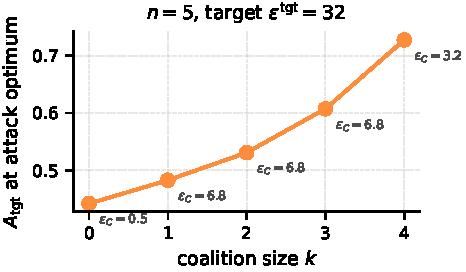
\includegraphics[width=\linewidth]{figures/fig_C4_coalition.pdf}
\caption{\textbf{C4.} Target's realised MIA advantage as a function of
coalition size $k$, with the coalition playing its target-maximising joint
action. Annotations show the optimal coalition budget $\eps^\star$ at each
$k$.}
\label{fig:C4}
\end{figure}

% =====================================================================
\subsection{C5 --- What is the functional form of the externality?}
\label{sec:C5}

\paragraph{Setup.} Two groups, target with budget $\eps_T \in \{4, 16\}$
fixed, others' budget $\eps_O$ swept over the log-spaced grid. The other
group's proportion of the total dataset is varied over
$\{0.2, 0.4, 0.6, 0.8\}$ at fixed total size $M = 10000$. This isolates the
target's vulnerability as a pure function of (a) what the others choose
and (b) how many of them there are.

\paragraph{Finding.} \emph{$A_t$ is monotone-decreasing in $\eps_O$; the
proportion-curves cross exactly at $\eps_O = \eps_T$.} \cref{fig:C5}: at
$\eps_T = 4$, $A_t$ ranges from $\approx 0.20$ (others at $\eps_O = 0.5$)
to $\approx 0$ (others at $\eps_O = 64$). At $\eps_T = 16$, the range is
$0.55$ down to $\approx 0.05$. For $\eps_O < \eps_T$ a larger proportion
of others raises $A_t$; for $\eps_O > \eps_T$ a larger proportion of
others lowers $A_t$. The crossover at $\eps_O = \eps_T$ is the regime in
which the others' choice and the target's choice contribute identically
to $\sigma$.

\paragraph{Implication.} This isolates the externality as a pure mechanism
effect, independent of any strategic choice. The shape mirrors Figure~3 of
\citet{kaiser2026your}, who showed the same dependence empirically through
the iDP-SGD trade-off function. C5 confirms that the externality lemma
(\cref{lem:externality}) is not just empirically monotone but
\emph{quantitatively} so: each unit decrease in others' $\eps$ corresponds
to a smooth, predictable increase in the target's realised $A$.

\begin{figure*}[!t]
\centering
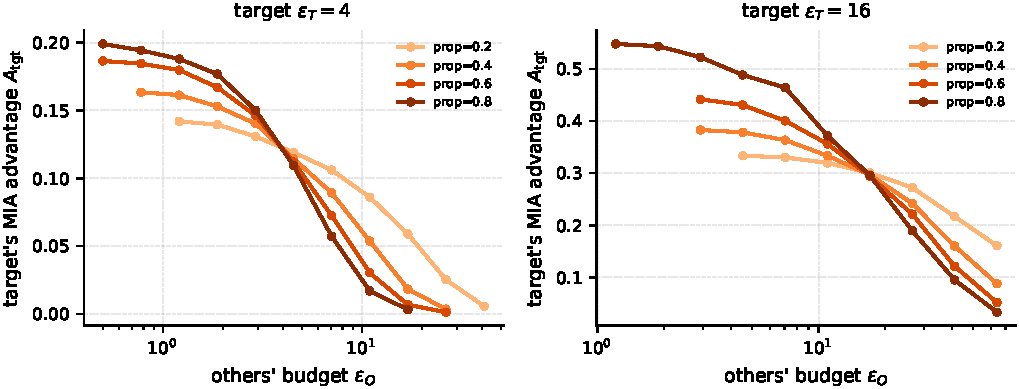
\includegraphics[width=\linewidth]{figures/fig_C5_surface.pdf}
\caption{\textbf{C5.} Target's realised MIA advantage as a function of the
other group's budget $\eps_O$ and proportion, at two fixed target budgets
$\eps_T \in \{4, 16\}$. The curves cross at $\eps_O = \eps_T$. Below
crossover, larger proportions raise $A_t$; above crossover, larger
proportions lower it.}
\label{fig:C5}
\end{figure*}

\section{Discussion and Conclusion}
\label{sec:discussion}

We have shown that sampling-based individual differential privacy is not just
\emph{vulnerable} to collusion attacks but \emph{equilibrium-incompatible}.
The pure Nash equilibria of the resulting game are intrinsically
\emph{asymmetric}---in the canonical $2$-player setting, both the naive
$(1, 8) / (8, 1)$ NE and the aware $(1, 2) / (2, 1)$ NE concentrate
vulnerability on one player while exempting the other. The budget-manipulation
attack of Kaiser et al.~\cite{kaiser2026your} is precisely the asymmetric naive
NE: a configuration that, by Proposition~\ref{prop:coalition-attack}, is the
rational best response of any coordinated subset of data holders, and that, by
Observation~\ref{obs:naive-ne}, is also reached by self-interested naive
players acting in isolation. The aware regime reduces the realised
population-level vulnerability by roughly $50\%$ but does \emph{not} restore
symmetry: it merely shifts the asymmetric equilibrium toward lower budgets.
The implication for designers of iDP systems is that the formal $(\eps_i,
\delta)$-iDP contract, while honoured at every individual record, will be
silently violated in the realised privacy of at least one of the contributors
in any pure Nash equilibrium of the strategic game it induces.

\paragraph{Limitations of this work.} Three caveats are worth noting.
First, our model assumes one-shot play. Real deployments of iDP are dynamic:
contributors join and leave; budgets can be re-negotiated; trainers
re-train. The repeated-game extension is the natural next step.
Second, we assume full information about other players' actions.
Real contracts may keep budgets private, so a Bayesian variant of the PEG
with private types is a natural and important direction. Third, our
analysis is restricted to the sampling-based realisation of iDP; the
\emph{sensitivity-based} realisation~\cite{boenisch2023have} adjusts per-sample
clipping bounds rather than per-sample sampling rates and does not exhibit the
same externality (the noise-to-sensitivity ratio is preserved by construction,
so privacy profiles are unaffected by the budget distribution). Our framework
specialises to that case as the trivial PEG in which the externality vanishes.

\paragraph{Mitigation.} The natural mitigation is to make the contract
internalise the externality. The $(\eps_i, \delta, \Delta)$-iDP formulation of
Kaiser et al.~\cite{kaiser2026your, kaissis2024beyond} adds a $\Delta$-divergence
bound on the realised vulnerability, restricting the action space of the PEG
to profiles that satisfy a per-record bound on excess advantage. We expect
this restriction to admit a unique equilibrium and to drive the Price of
Excess Vulnerability to zero (by definition). Characterising the constrained
PEG and identifying its equilibrium is a clean extension of this work.

\paragraph{Wider lesson.} The wider lesson of this paper is that an
\emph{individual} privacy contract is incomplete: it does not pin down the
collective dynamics. Where individuals interact strategically (in a single
machine-learning training, in a federated round, in any future composition of
the iDP mechanism), the contract must also constrain their joint behaviour or
the equilibrium will quietly violate every participant's expectations while
preserving every formal guarantee. The Privacy Externality Game makes this
gap explicit, formalises the equilibrium, and clarifies what an iDP contract
must do to close it.

\paragraph{Conclusion.} The promise of iDP---that every data contributor
controls her own privacy---is broken by the privacy externality of sampling-
based mechanisms. We formalised the strategic situation faced by iDP data
contributors as the Privacy Externality Game, proved monotonicity of the
externality and characterised the equilibria. The result is that the
collusion attack on iDP is not adversarial but \emph{rational}, and the
remedy must operate at the level of the contract.


\bibliographystyle{IEEEtran}
\bibliography{refs}

\appendices

\section{Detailed mechanism-solver construction}
\label{app:mechanism}

We elaborate on the bisection used to obtain the mechanism solution
$(\sigma, p_1,\dots,p_n)$ for an action profile $\boldsymbol{\eps}$.

\paragraph{Inner step: $p_g$ from $(\sigma, \eps_g)$.}
For each fixed $\sigma$ and each group~$g$, we want the largest $p_g \in [0, 1]$
satisfying the $I$-fold $(p_g, \sigma)$-subsampled Gaussian
at $(\eps_g, \delta)$-DP under (C1). Since the $\eps$ value of the
subsampled Gaussian is strictly increasing in $p_g$ (more sampling
$\Rightarrow$ more privacy loss), a unique $p_g \in (0, 1]$ exists, capped at
$1$ if the budget cannot be exhausted. We compute the per-group $\eps$ by
R\'enyi-DP composition~\cite{mironov2017renyi} (which gives an upper bound that
binds in the regime of interest) and binary-search $p_g$ to bring this $\eps$
to $\eps_g$ to within a relative tolerance of $10^{-3}$.

\paragraph{Outer step: $\sigma$ from $(p_g, \boldsymbol{\eps})$.}
Define $B(\sigma) = \sum_g |G_g|\, p_g(\sigma, \boldsymbol{\eps})$ as the
realised expected batch size. Since each $p_g$ is monotone-increasing in
$\sigma$, so is $B$. We bisect $\sigma$ to bring $B$ to the target $E_b$,
again to within a relative tolerance of $10^{-3}$.

\paragraph{MIA advantage.}
Given the mechanism solution $(\sigma, p_g)$, we compute the MIA advantage of
group~$g$ from the privacy-loss-distribution of the $I$-fold $(p_g, \sigma)$-
subsampled Gaussian using \cite{google-dp-accounting}, then evaluate the
trade-off function and \cref{eq:adv}:
\begin{equation}
A_g \;=\; \sup_\alpha \,\bigl(1 - \alpha - T_g(\alpha)\bigr),
\quad
T_g(\alpha) \;=\; \sup_{\eps \geq 0} \,\bigl(1 - \delta_g(\eps) - \alpha \cdot e^\eps\bigr)^+.
\end{equation}
This is the formulation of Kaiser et al.~\cite{kaiser2026your} and gives the
tightest analytical MIA advantage for the resulting mechanism.

\section{Caveats on the equilibrium reporting}
\label{app:caveats}

\paragraph{Cycling in the aware regime.}
The aware-regime PEG has utility functions that mix a (globally shared)
$V(\sigma)$ term with a (player-specific) $A_i(\boldsymbol{\eps})$ term. The
sign of the cross-partials $\partial^2 u_i / \partial \eps_i \partial \eps_j$ is
not constant on the action grid: at low $\eps_i$, lowering $\eps_j$
\emph{decreases} $V$ (penalises both players), but at high $\eps_i$ it
mostly steers $A_i$ upward (penalises player $i$ more). The result is a
non-supermodular game which admits no pure NE in general. Our experiments
report the BR-cycle average as a stand-in for an empirical mixed equilibrium.

\paragraph{Sensitivity to the action grid.}
The choice of action grid $\mathcal{A}$ matters: a coarse grid yields a coarse
equilibrium. We use $\mathcal{A} = \{1, 2, 4, 8, 16, 32, 64\}$ throughout. A
sensitivity check with a finer grid (powers of $\sqrt{2}$ between $1$ and $64$)
yields qualitatively identical curves with smoother transitions.

\paragraph{Choice of $V$ and $C$.}
We use $V(\sigma) = 1/(1+\sigma)$ and $B_i = C_i = 1$. Pej\'o et
al.~\cite{pejo2019together} use linear $V$. Our results are qualitatively
unchanged under either choice provided $V$ is strictly decreasing and convex
in $\sigma$.


\end{document}
